\subsection{Osmanlılar Galerisi}
\indent\indent Müzede en büyük kısım Osmanlı dönemi eserlerine ayrılmıştır. Bu salonda ağırlıklı olarak Osmanlı dönemi kilimleri ve halıları bulunmaktadır. Bu halı ve kilimler arasında Holbein, Lotto ve Bellini isimleri göze çarpmaktadır. Mezkur ressamlar, eserlerinde Türk halılarını resmettiğinden dolayı, benzer motifli halılar ressamların isimleri ile anılmaktadır. 15. ve 16.yüzyılda halı kullanımı Avrupa'da yaygın olmadığı için, bu halıları zaman zaman masaların üzerine serilmiş şekilde görebiliyoruz resimlerde. Holbein halılarının ana özelliği, sekizgen şeklinde madalyonları ihtiva etmesidir. Hans Holbein'in eseleri ve müzedeki halıların karşılaştırması aşağıda görülebilir. (Şekil \ref{fig:holbein})\newline
\begin{figure}[H]
    \centering
    \subfigure[Somerset Ev Konferansı(1604) - Hans Holbein]{
        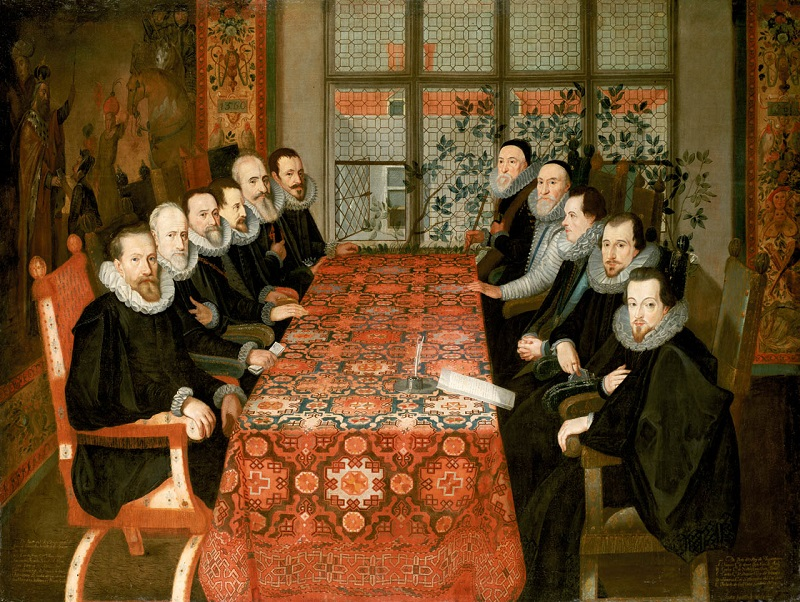
\includegraphics[height=0.3\textheight,width=0.45\linewidth]{assets/somerset_house_conference.jpg}
    }
    \subfigure[Elçiler - Hans Holbein]{
        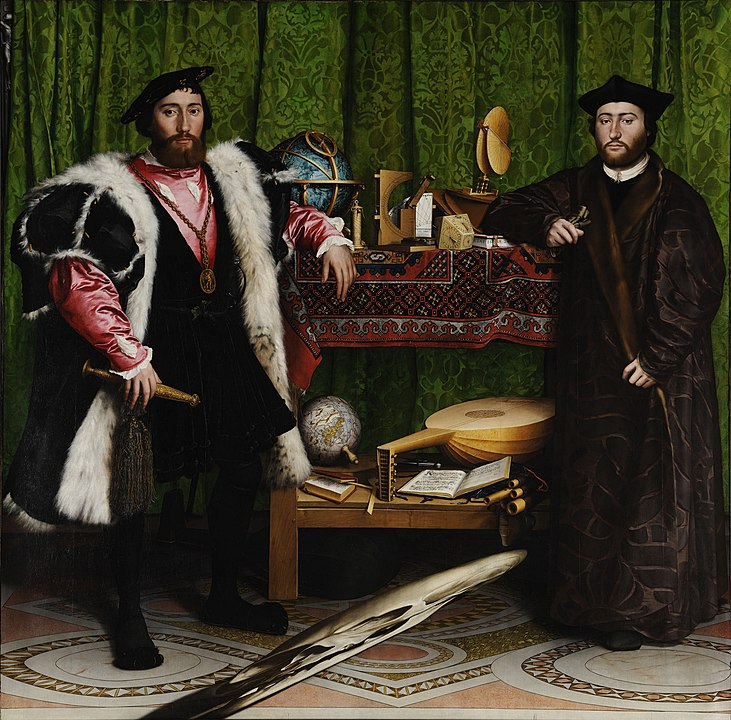
\includegraphics[height=0.3\textheight,width=0.45\linewidth]{assets/envoy.jpg}
    }
    \subfigure[Holbein Halısı - 1]{
        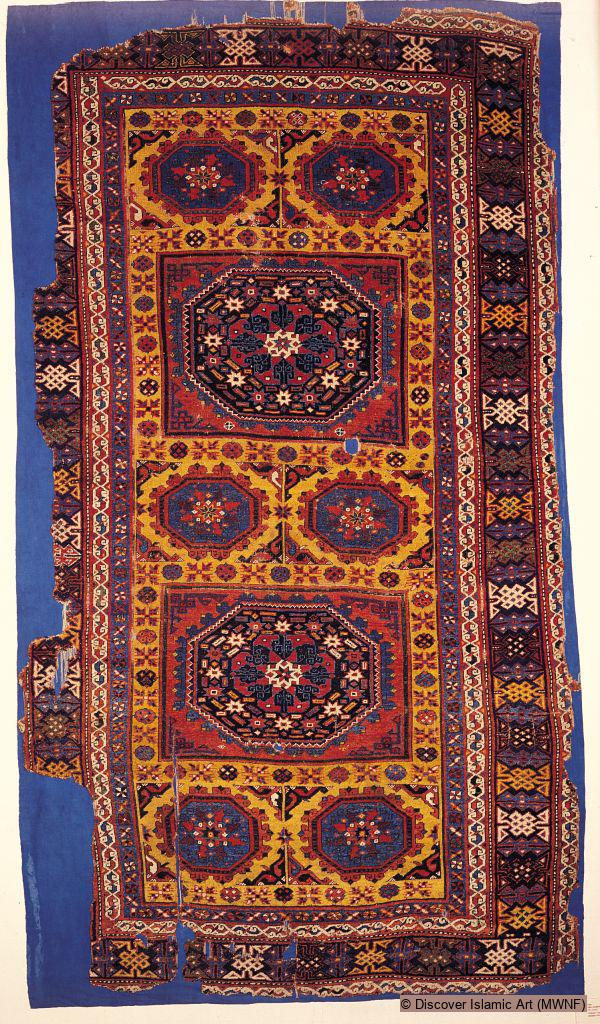
\includegraphics[height=0.3\textheight,width=0.30\linewidth]{assets/holbein_1.jpg}
    }
    \subfigure[Holbein Halısı - 2]{
        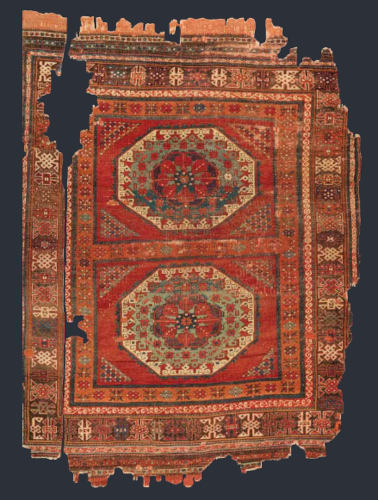
\includegraphics[height=0.3\textheight,width=0.30\linewidth]{assets/holbein_2.png}
    }
    \subfigure[Holbein Halısı - 3]{
        \includegraphics[height=0.3\textheight,width=0.30\linewidth]{assets/holbein_3.jpg}
    }
    \caption{Holbein Resimleri ve Halıları Karşılaştırmalı}
    \label{fig:holbein}
\end{figure}
\indent Yine bu salonda Osmanlı dönemi el yazması eserler, fermanlar ve kuburlar sergilenmektedir. El yazması eserler arasında en ilgi çekici olanı ise \textit{Zübdetü't Tevârîh} isimli eserdir. Eser, III. Murad döneminin Şehnamecisi olan Seyid Lokman Aşuri tarafından yazılmıştır. Eserde, peygamberler ve hükümdarların yaşamlarında vuku bulmuş önemli tarihi olaylar anlatılmış ve minyatür şeklinde resmedilmiştir. III.Murad'a kadar olan bütün Osmanlı padişahlarına da yer veilmiştir. Eserin açık sayfasındaki minyatürde Hz.Yakup ve Hz.Yusuf'un kavuşması ve  on bir kardeşi ile onan inanaların bulunduğu meclis resmedilmiştir.\newline
\begin{figure}[H]
    \centering
    \subfigure[Ferman ve Kuburlar]{
        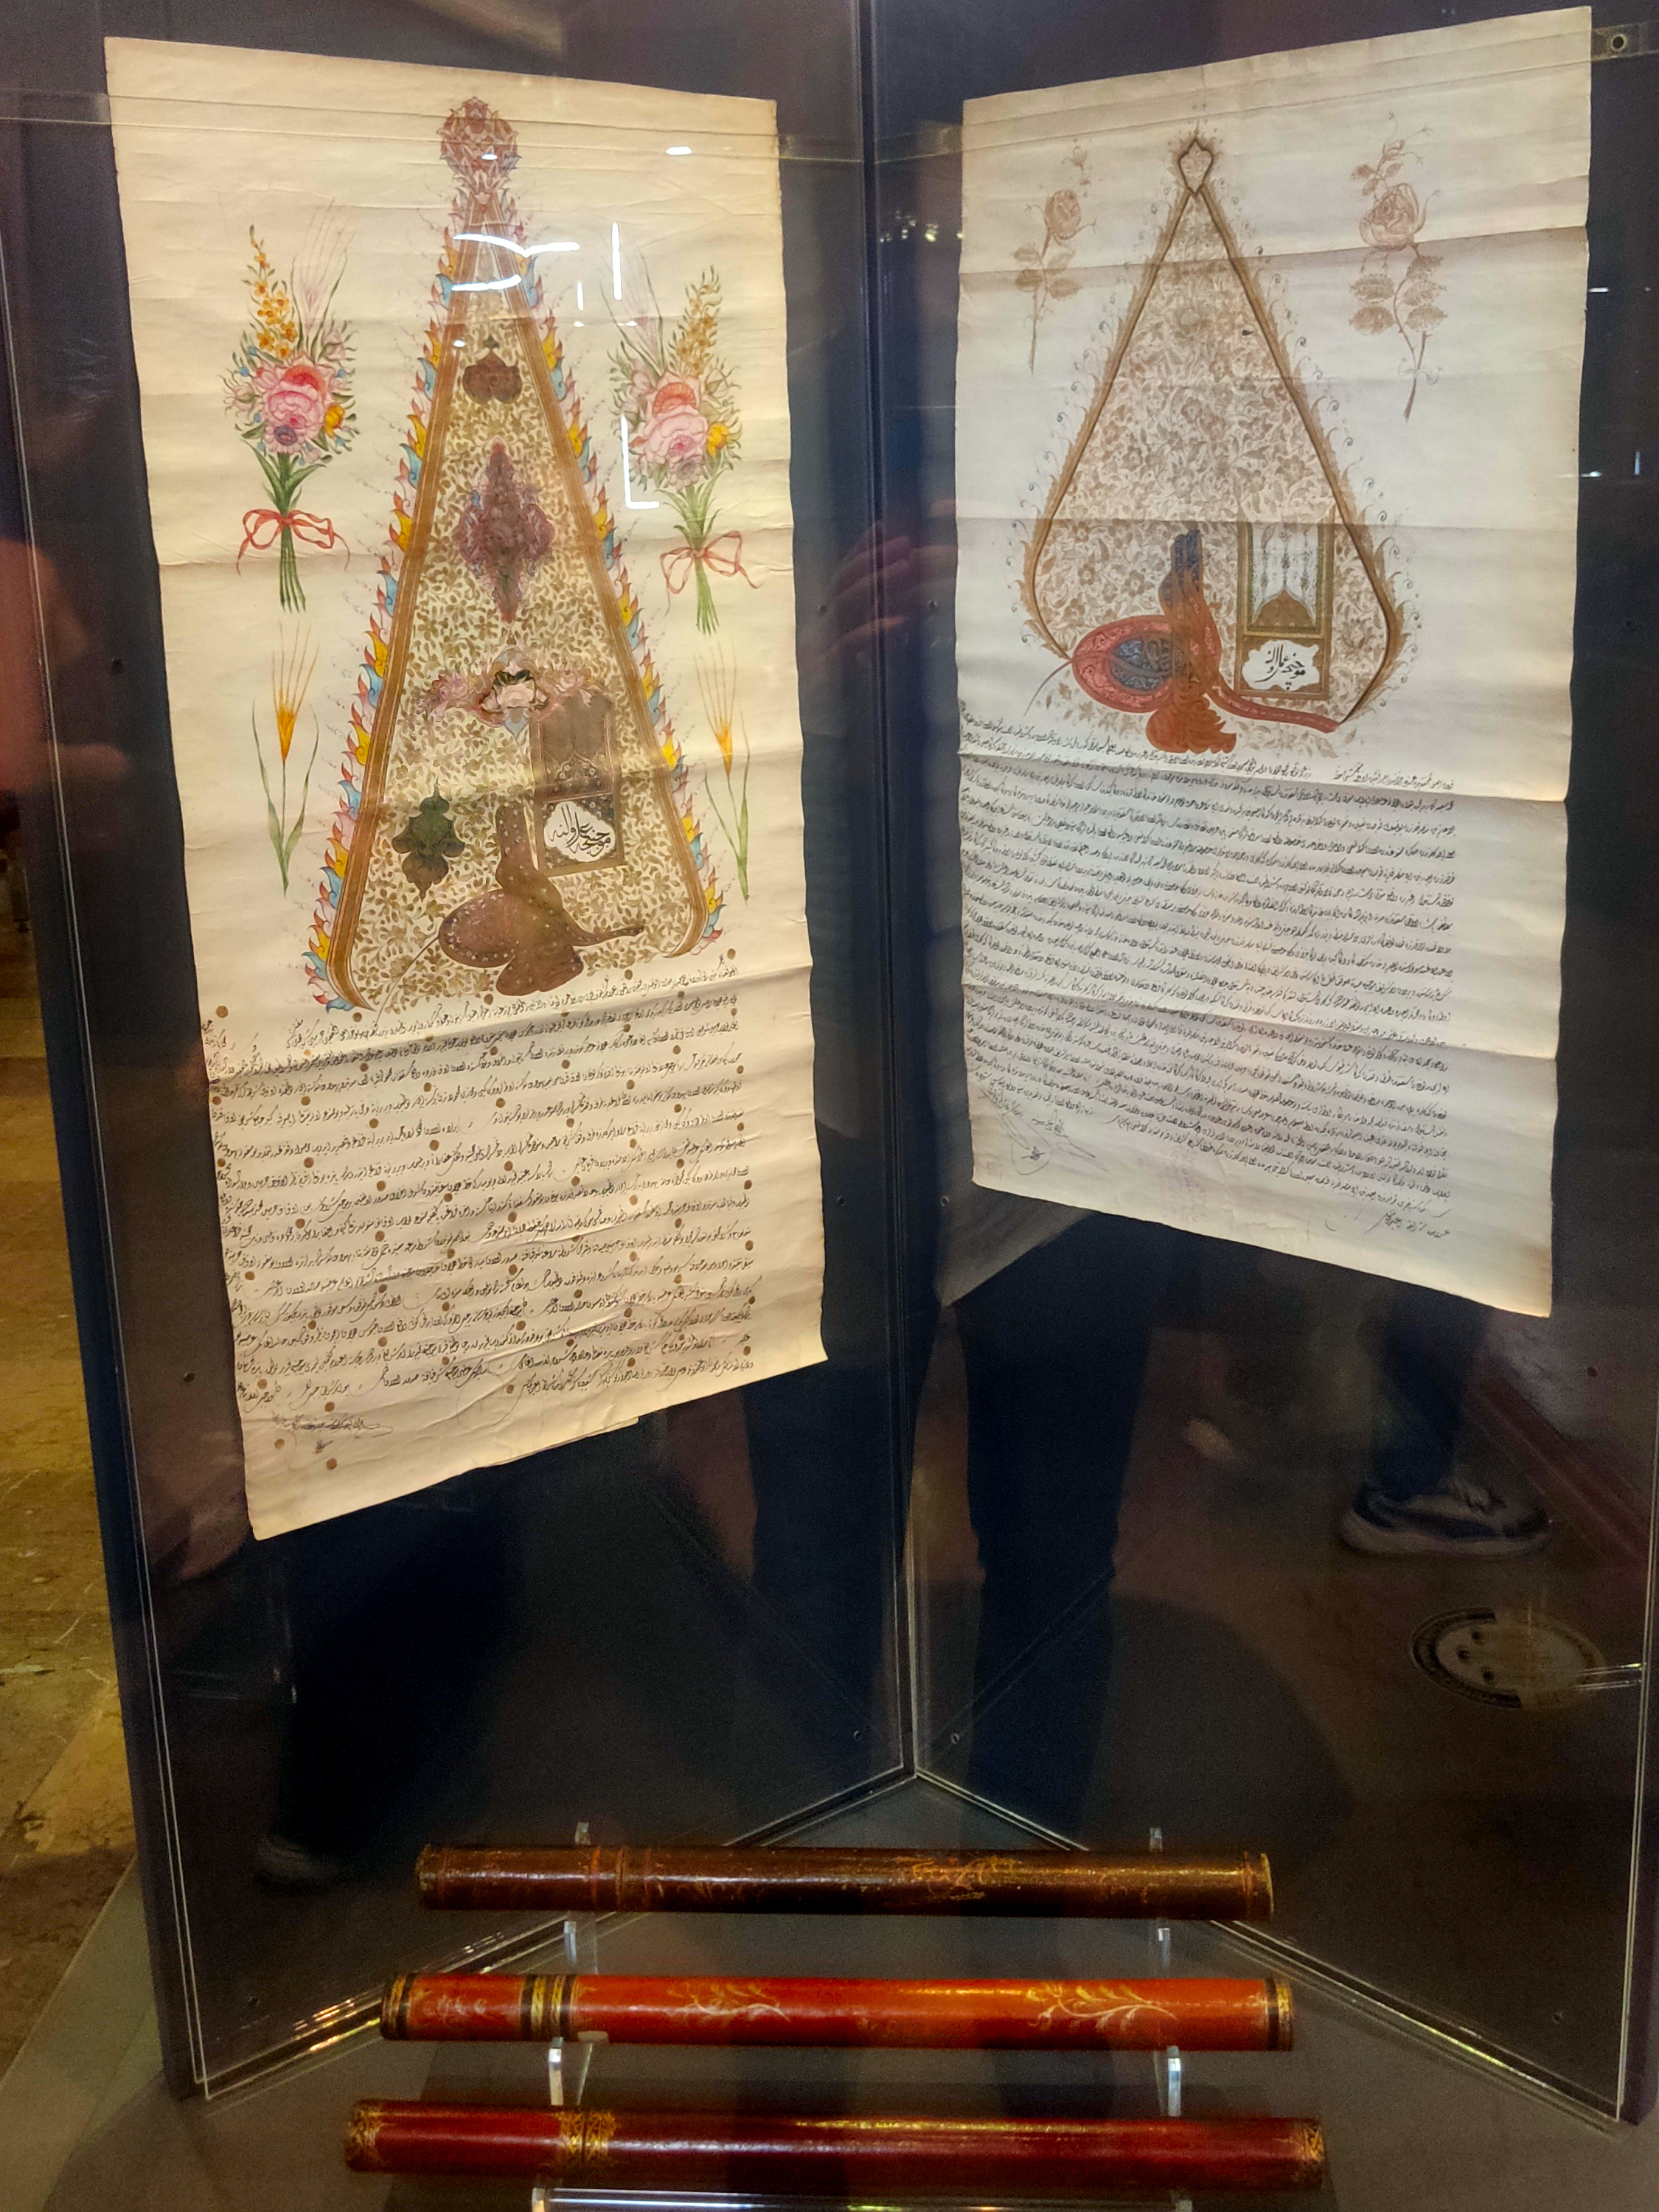
\includegraphics[height=0.25\textheight]{assets/kubur.jpg}
    }
    \subfigure[Zübdetü't Tevârîh]{
        \includegraphics[height=0.25\textheight]{assets/zubdetut_tevarih.jpg}
    }
    \caption{El Yazması Eserler}
\end{figure}
\indent Bu eserlere ek olarak, Osmanlı hanedanına ait mücheveler ve takılar da bu salonda incelenebilir. Bunlar arasında Hürrem Sultan'ın takıları öne çıkan eserlerden biridir. Hanedan ailesi tarafından kullanılmış altın ve yakut işlemeli kemerler bu kısımda sergilenmektedir.
\begin{figure}[H]
    \centering
    \subfigure[Takılar]{
        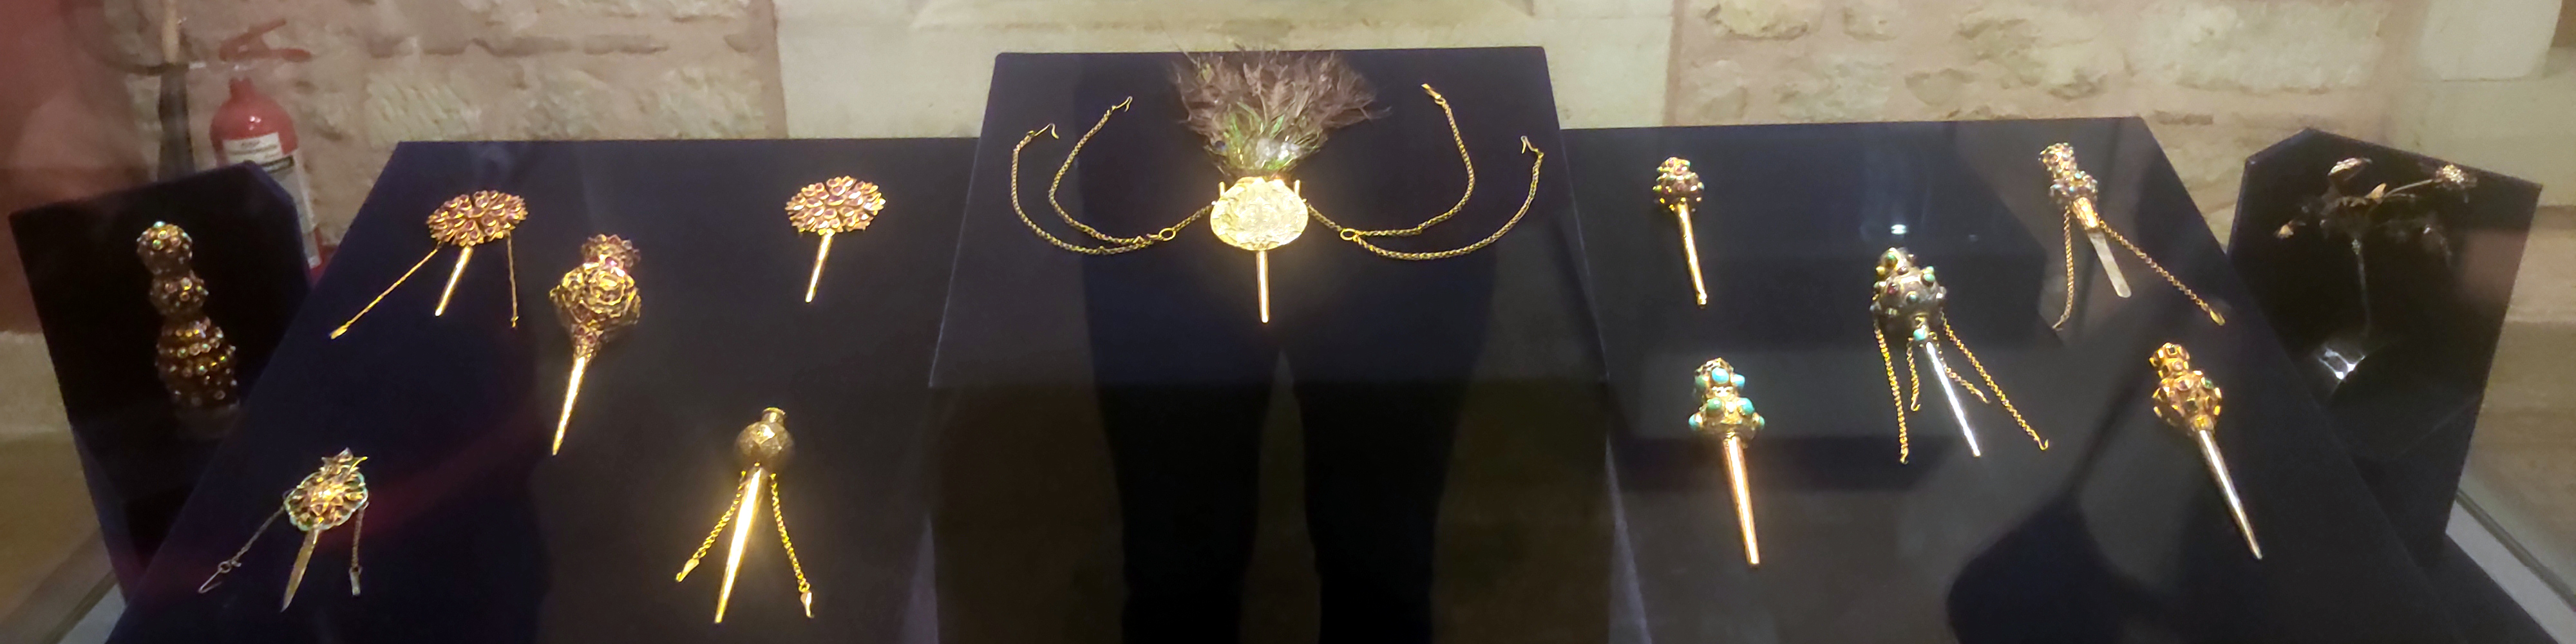
\includegraphics[width=0.9\linewidth]{assets/jewelry.jpg}
        \label{fig:jewelry}
    }
    \subfigure[Mücheverler ve Takılar]{
        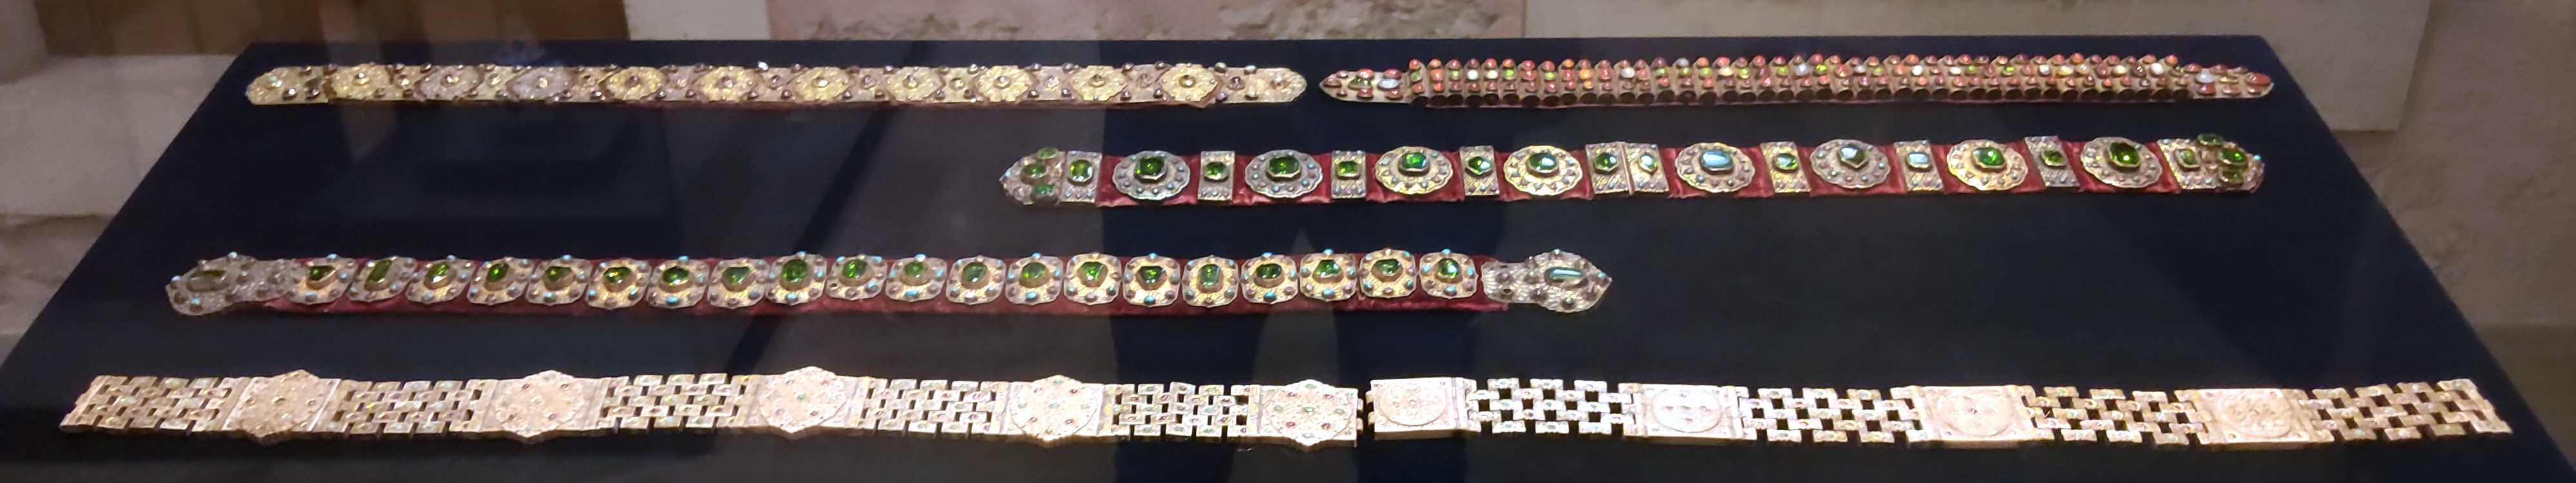
\includegraphics[width=0.9\linewidth]{assets/belts.jpg}
        \label{fig:belts}
    }
    \caption{Hanedan Takıları ve Kemerleri}
\end{figure}